\documentclass{article}
\usepackage{graphicx} % Required for inserting images

\usepackage{darkmode}
\enabledarkmode 
\usepackage{amsmath}
\usepackage{tikz}
\usepackage{framed}
\usepackage{pgfplots}
\usepackage{pgfplotstable}
\usetikzlibrary{3d, positioning}


\begin{document}
    \section{Center of Mass}
        \subsection{Discrete}
        \begin{equation}
            \large
            R_{cm} = \frac{1}{M_{total}} \sum_{n=1}^{N} m_n r_n
        \end{equation}
        \hfil

        Find a point in the center of a group of points. 

        \subsubsection{Example one}
        \begin{center}
            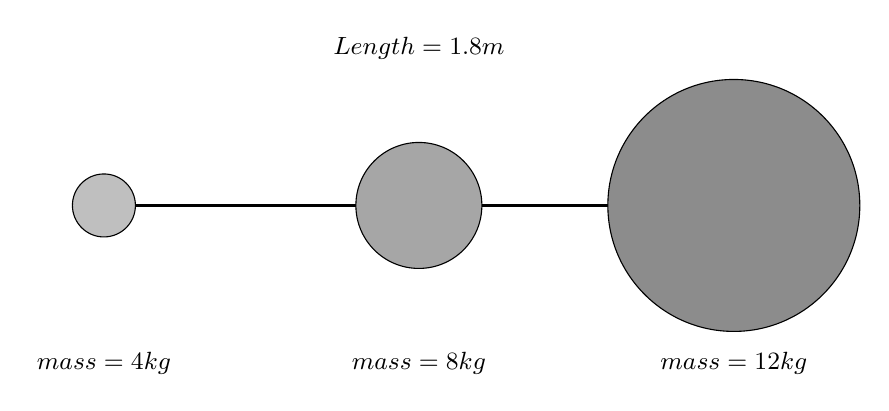
\begin{tikzpicture}[scale=.4]
                % Define the positions
                \draw[thick] (-10,0) -- (10,0); % Draw a horizontal reference line
                
                % Draw circles with specified radii
                \draw[fill=gray!50] (-10, 0) circle (1);  % First ball with radius 4
                \draw[fill=gray!70] (0, 0) circle (2);   % Second ball with radius 8
                \draw[fill=gray!90] (10, 0) circle (4);  % Third ball with radius 12
            
                % Labels for clarity
                \node at (-10, -5) {\small $mass=4kg$};
                \node at (0, -5) {\small $mass=8kg$};
                \node at (10, -5) {\small $mass=12kg$};
                \node at (0, 5) {\small $Length = 1.8m$};

            \end{tikzpicture}
        \end{center}
        \[\boxed{x_{cm} = \frac{x_1m_1 + x_2m_2+ x_3m_3 }{m_1+ m_2 + m_3}}\]

        \[\boxed{x_{cm} = \frac{(0)(4) + (.9)(8) + (1.8)(12) }{4 + 8 + 12}}\]
        

        \subsubsection{Example Two}
            \begin{center}
                \begin{tabular}{|| c c c c c ||}
                    \hline
                    m & x & y & $v_x$ & $v_y$  \\ 
                    \hline
                    1 & 7.8 & -2.8 & 3.2 & -4.2 \\  
                    2 & 7.8 & -3.7  & -5.2 &  5.2 \\
                    3 & 7.8 & -5.7  & -6.2 &  2.2 \\ 
                    4 & 7.8 & 2.7  & 4.2 & -3.2 \\
                    \hline
                \end{tabular}
            \end{center}
        
           \[\boxed{x_{cm} = \frac{x_1m_1 + x_2m_2+ x_3m_3 + x_4m_4}{m_1+ m_2 + m_3 +m_4}}\]


        \subsection{Example Three}

            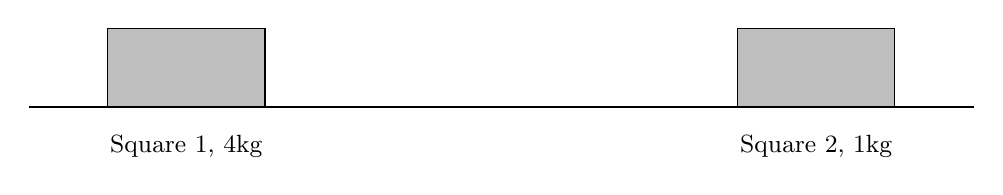
\begin{tikzpicture}
                % Draw a horizontal reference line
                \draw[thick] (-6,0) -- (6,0);
                
                % Draw two squares, 10 units apart
                
                \draw[fill=gray!50] (-5,0) rectangle (-3,1); % First square
                \draw[fill=gray!50] (3,0) rectangle (5,1);   % Second square
                
                % Labels
                \node at (-4, -.5) {\small Square 1, 4kg};
                \node at (4, -.5) {\small Square 2, 1kg};
            \end{tikzpicture}
     
        \pagebreak



        \subsection{Continuous}
        \[R_{cm} = \frac{1}{M_{total}} \int \vec{r}dm\]

        \subsection{COM of multiple objects}


    \pagebreak
    \section{Momentum}

    \begin{equation}
        \huge
        \boxed{\vec{P} = m\vec{v}}
    \end{equation}
    
    Different version of Newtons law.
    \subsection{Eleastic Collisons}
        \begin{list}{-}{}
            \item Conservation of linear Momentum
            \item conservation of mechanical energy
            \item kinetic energy of the system is conserved, 
            \item kinetic energy of the individual bodies can change
            \item ex. Billiard ball collisions
        \end{list}
    \subsection{Inelastic Collisions}
        \begin{list}{-}{}
            \item Mechanical energy not conserved 
            \item conservation of linear Momentum
            \item loss of energy: sound, heat, Elastic, Etc 
            \item bodies stick together 
            \item paintball
        \end{list}

    In a closed system, no momentum will be  lost. 

    \begin{list}{-}{}
        \item Friction is typically not considered 
        \item typically the system will have a net force
    \end{list}
\end{document}